\section{Proposed Methodology}
\subsection{Pipeline Overview}
Fig.~\ref{fig:pipeline} shows the MultiCardioFusion pipeline. The clinical table (D1) is enriched with ECG-proxy features derived from the same patients' resting-ECG and exercise-test measurements (D3, Section~IV-D). Feature fusion with tree ensembles, a soft-voting ensemble and dual-branch neural networks are then trained and compared, and TreeSHAP explains the XGBoost member \emph{post hoc}. The PTB-XL branch (D2) is trained and evaluated separately with its own labels (Table~\ref{tab:mapping}).

\begin{figure}[!t]
\centering
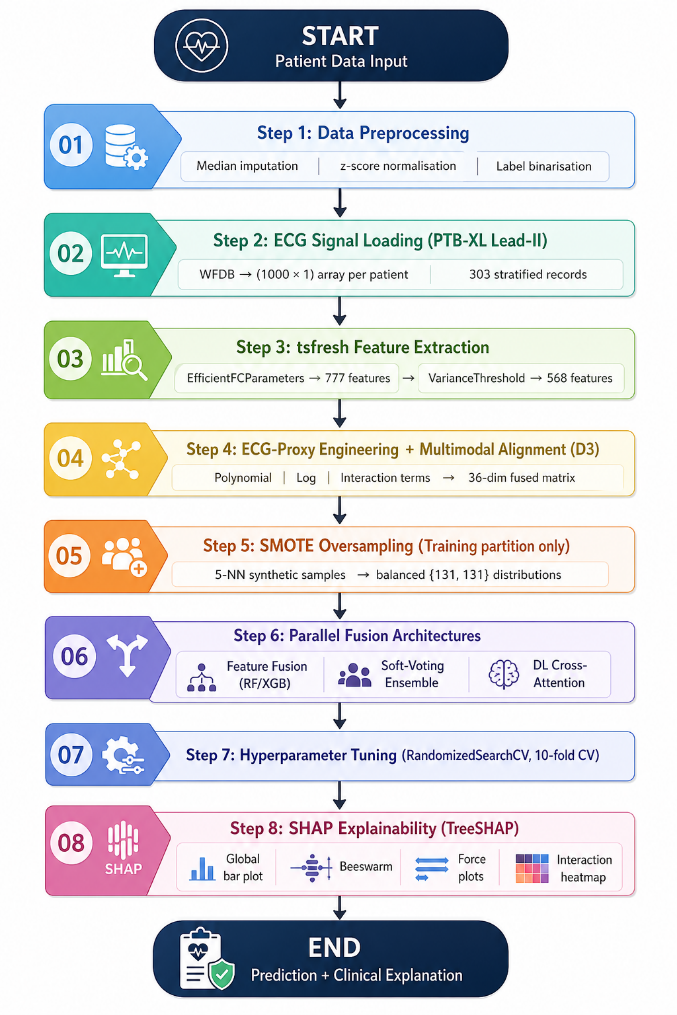
\includegraphics[width=0.78\linewidth]{fig2_pipeline.png}
\caption{MultiCardioFusion pipeline (as in v4). In this revision steps 1, 3, 4 and 5 are fitted inside each training fold (Algorithm~\ref{alg:train}).}
\label{fig:pipeline}
\end{figure}

\subsection{Algorithms}
The single MCF-BiModNet algorithm of v4 mixed a network forward pass with resampling, ensembling and explanation, which happen at different stages. It is split here into three algorithms: feature construction (Alg.~\ref{alg:proxy}), training and evaluation (Alg.~\ref{alg:train}) and post-hoc explanation (Alg.~\ref{alg:shap}). SHAP is \emph{not} part of prediction.

\begin{algorithm}[!t]
\caption{ECG-proxy feature construction (row-wise, no fitted parameters)}
\label{alg:proxy}
\begin{algorithmic}[1]
\Require imputed clinical vector $x\in\mathbb{R}^{13}$
\State $e \gets (\text{restecg}, \text{oldpeak}, \text{slope}, \text{thalach}, \text{exang})$ \Comment{5 raw ECG-linked}
\State append polynomial, interaction, log, ratio, threshold, HR-reserve and ischaemia terms (Section~IV-D) \Comment{18 derived}
\State \Return $[x;\, e] \in \mathbb{R}^{36}$
\end{algorithmic}
\end{algorithm}

\begin{algorithm}[!t]
\caption{Training and evaluation (repeated stratified CV)}
\label{alg:train}
\begin{algorithmic}[1]
\Require raw data $(X, y)$ with missing values; $R$ repeats, $K$ folds; fixed hyper-parameters $\theta$
\For{$r = 1..R$, $k = 1..K$}
  \State split into training $\mathcal{T}$ and test $\mathcal{V}$ (stratified)
  \State fit median imputer on $\mathcal{T}$; apply to $\mathcal{T}, \mathcal{V}$
  \State build features with Alg.~\ref{alg:proxy}; fit StandardScaler on $\mathcal{T}$
  \State resample $\mathcal{T}$ only (e.g.\ SMOTE, $k=5$)
  \State fit XGB, SVM, GBM, RF with $\theta$; $\bar P(x)=\frac14\sum_m P_m(x)$
  \State record AUC, accuracy, sensitivity, specificity, F1, Brier on $\mathcal{V}$
\EndFor
\State \Return fold metrics and paired differences with corrected CIs (Section~IV-G)
\end{algorithmic}
\end{algorithm}

\begin{algorithm}[!t]
\caption{Post-hoc interpretation (not used for prediction)}
\label{alg:shap}
\begin{algorithmic}[1]
\Require fitted XGBoost member $f$, transformed test features $Z_{\mathcal{V}}$
\State $\phi \gets \text{TreeSHAP}(f, Z_{\mathcal{V}})$; global importance $\bar\phi_j=\text{mean}|\phi_{\cdot j}|$
\State repeat over folds and seeds; report rank stability and agreement with permutation importance
\end{algorithmic}
\end{algorithm}

\subsection{Mathematical Formulation}
\textbf{SMOTE.} For a minority sample $x_i$, SMOTE~\cite{chawla2002} creates $\tilde x = x_i + \lambda(\hat x - x_i)$ with $\hat x$ one of the $k=5$ nearest minority neighbours and $\lambda\sim U(0,1)$. Interpolation stays within the convex hull of observed patients, but on mixed data it produces non-integer categorical codes and, when applied after feature derivation, derived features that no longer match their inputs (Section~VI-C). We therefore also evaluate SMOTE-NC~\cite{chawla2002} and resampling of the raw rows before feature derivation.

\textbf{Cross-attention with sequence length 1.} MCF-BiModNet reshapes each 32-dimensional branch output to a sequence of length $L=1$ and applies $\mathrm{Attention}(Q,K,V)=\mathrm{softmax}(QK^\top/\sqrt{d_k})V$ with $Q=W_Q h_{\text{ecg}}$, $K=W_K h_{\text{clin}}$, $V=W_V h_{\text{clin}}$. With one key, the softmax is taken over a single score, so the attention weight is exactly 1 for every head and every input. The block therefore reduces to
\begin{equation}
\mathrm{MultiHead}(h_{\text{ecg}}, h_{\text{clin}}) = W_O\,(W_V h_{\text{clin}} + b_V) + b_O ,
\end{equation}
a linear map of the clinical branch that does not depend on the ECG ``query''. We verify this numerically and compare the architecture with an explicit linear layer and with a \emph{token-level} variant in which every feature is a token, so that ECG-proxy tokens attend over 13 clinical tokens and the softmax is non-trivial (Section~VI-I).

\textbf{Soft voting.} Each base classifier $c_m$ outputs $P_m(x)\in[0,1]$; the ensemble predicts $\bar P(x) = \frac1M\sum_m P_m(x)$ and $\hat y = \mathbb{1}[\bar P(x)\geq 0.5]$. We compare soft voting with hard voting and with stacking, whose logistic meta-learner learns the member weights.

\textbf{TreeSHAP.} $\phi_j = \sum_{S\subseteq F\setminus\{j\}} \frac{|S|!(|F|-|S|-1)!}{|F|!}\,[f(S\cup\{j\}) - f(S)]$, computed exactly for tree ensembles in $O(TLD^2)$~\cite{lundberg2018tree}.

\subsection{ECG-Proxy Feature Engineering}
From the five ECG-related Cleveland variables (restecg, oldpeak, slope, thalach, exang) we derive 18 additional terms:
\emph{polynomial} oldpeak$^2$, thalach$^2$;
\emph{interactions} oldpeak$\times$slope, thalach$\times$exang, oldpeak$\times$thalach, restecg$\times$oldpeak, slope$\times$thalach;
\emph{log} $\log(1+\text{oldpeak})$, $\log(\text{thalach})$;
\emph{ratios} oldpeak/thalach, thalach/slope;
\emph{threshold flags} oldpeak$>$1, thalach$<$140, restecg$>$0, ``downslope'';
\emph{heart-rate reserve} thalach$-(220-\text{age})$ and its ratio to $220-\text{age}$;
and an \emph{ischaemia score} oldpeak$\cdot$(slope$+$1)$+$2$\cdot$exang.
Together with the five raw variables this gives a 23-column ECG-proxy block and a 36-column matrix D3. Two properties matter for interpretation. First, the five raw columns are exact copies of clinical columns, so D3 contains duplicates. Second, the v4 code defines ``downslope'' as slope $=2$, which in UCI coding is a \emph{flat} slope (downsloping is 3). Both are tested in Section~VI-A.

\subsection{Classifiers and Hyper-Parameters}
All models were implemented with scikit-learn~\cite{pedregosa2011}, XGBoost and imbalanced-learn~\cite{lemaitre2017}. The four ensemble members were tuned once by RandomizedSearchCV (10-fold) on the v4 training split: XGBoost~\cite{chen2016} (200 trees, depth 3, learning rate 0.01, column subsample 0.7), RBF-SVM~\cite{cortes1995} ($C=100$, $\gamma=0.001$), gradient boosting (200 trees, depth 3, learning rate 0.01) and random forest~\cite{breiman2001} (500 trees, depth 20, $\log_2$ features). In every experiment of Section~VI these values are \emph{fixed}, so all variants share the same tuning budget. Because they were tuned on data that overlaps the CV test folds, we also report fully nested tuning (Section~VI-D).

\subsection{Dual-Branch Neural Networks}
Each branch is Dense(64, ReLU)$\rightarrow$BatchNorm$\rightarrow$Dropout(0.4)$\rightarrow$Dense(32, ReLU)~\cite{ioffe2015,srivastava2014}. The clinical branch receives the 13 clinical columns and the ECG branch the 23 proxy columns. The branches are combined by concatenation, by multi-head cross-attention with $L=1$ (4 heads, $d_k=8$, residual to the ECG branch; the v4 architecture), by a linear layer (its equivalent), or by token-level cross-attention, in which each feature is embedded as its own token as in the FT-Transformer~\cite{gorishniy2021}. A Dense(16, ReLU)$\rightarrow$sigmoid head follows. Training uses Adam~\cite{kingma2015} (learning rate $10^{-3}$, batch 16, at most 200 epochs) with early stopping (patience 15, best weights restored) and learning-rate halving (patience 7) on a 20\% validation split of the training fold. \revnote{Note: the v4 notebook trained only a clinical-only MLP, so the cross-attention results reported in v4 had no corresponding code; the networks evaluated here were implemented for this revision.}

\subsection{Evaluation Protocol}
\textbf{Primary protocol.} All results in Section~VI use repeated stratified 10-fold CV with $R=5$ repeats (50 folds; 30 folds for the costlier neural and robustness experiments), with identical splits for every variant (Algorithm~\ref{alg:train}). AUC is the primary metric; sensitivity matters most clinically because a missed CAD case costs more than a false alarm. We also report specificity, F1, the Brier score and the calibration slope (ideal 1)~\cite{vancalster2019}.

\textbf{Uncertainty and tests.} Fold scores from repeated CV are not independent because training sets overlap, and a naive $t$-interval is too narrow. For a metric or paired difference $d_1,\dots,d_n$ over $n$ folds we use the corrected resampled $t$-statistic of Nadeau and Bengio~\cite{nadeau2003,bouckaert2004}:
\begin{equation}
t=\frac{\bar d}{\sqrt{\left(\frac1n+\frac{n_{\text{test}}}{n_{\text{train}}}\right)\hat\sigma^2_d}},
\end{equation}
with $n-1$ degrees of freedom and $n_{\text{test}}/n_{\text{train}}=1/9$, and report the matching 95\% CI. P-values within a table are adjusted with the Holm procedure~\cite{holm1979}. For external sites and subgroups we use 2{,}000 bootstrap resamples of patients. A label-permutation test~\cite{ojala2010} checks performance against chance.

\textbf{Hold-out.} For comparability with v4 we also report the 80/20 stratified hold-out (242/61 patients, seed 42), and its sensitivity to the choice of split (Section~VI-D).
